\section{MAESTRO Basics}

MAESTRO models problems that are in tight hydrostatic equilibrium.
The fluid state is decomposed into a 1-d radial base state that
describes the hydrostatic structure of the star or atmosphere, and a
2- or 3-d Cartesian full state, that captures the departures from
hydrostatic equilibrium.  Two basic geometries are allowed.  A {\em
  plane-parallel} geometry assumes that the domain is thin compared to
the radius of curvature of the star, and therefore the 1-d base state
is perfectly aligned with the Cartesian state.  A {\em spherical}
geometry is for modeling an entire star.  Here, the 1-d base state is
not aligned with the Cartesian state.  Figure~\ref{fig:base_state}
shows these geometries.

\begin{figure}[tb]
\centering
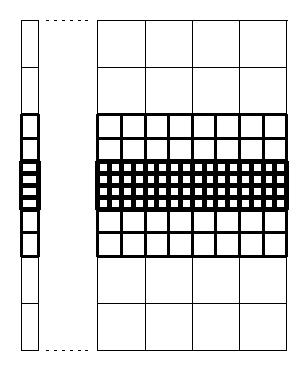
\includegraphics[height=2.0in]{\archfigpath/base_grid} \hspace{0.5in}
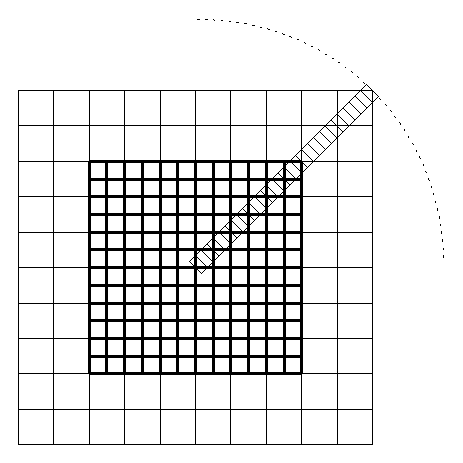
\includegraphics[height=2.0in]{\archfigpath/base_spherical}
\caption{\label{fig:base_state} MAESTRO geometries, showing both the
  1-d base state and the full Cartesian state.  (Left) For multi-level
  problems in planar geometry, we force a direct alignment between the
  radial array cell centers and the Cartesian grid cell centers by
  allowing the radial base state spacing to change with space and
  time.  (Right) For multi-level problems in spherical geometry, since
  there is no direct alignment between the radial array cell centers
  and the Cartesian grid cell centers, we choose to fix the radial
  base state spacing across levels. Figure taken
  from~\cite{multilevel}.}
\end{figure}


MAESTRO can use adaptive mesh refinement to focus resolution on
complex regions of flow.  For Cartesian/plane-parallel geometries, all
cells at the same height must be at the same level of refinement.
This restriction is to allow for the base state to directly align with
the Cartesian state everywhere.  For spherical geometries, there is no
such restriction (again, see Figure~\ref{fig:base_state}).




\section{MAESTRO Directory Structure}

\begin{figure}[t]
\centering
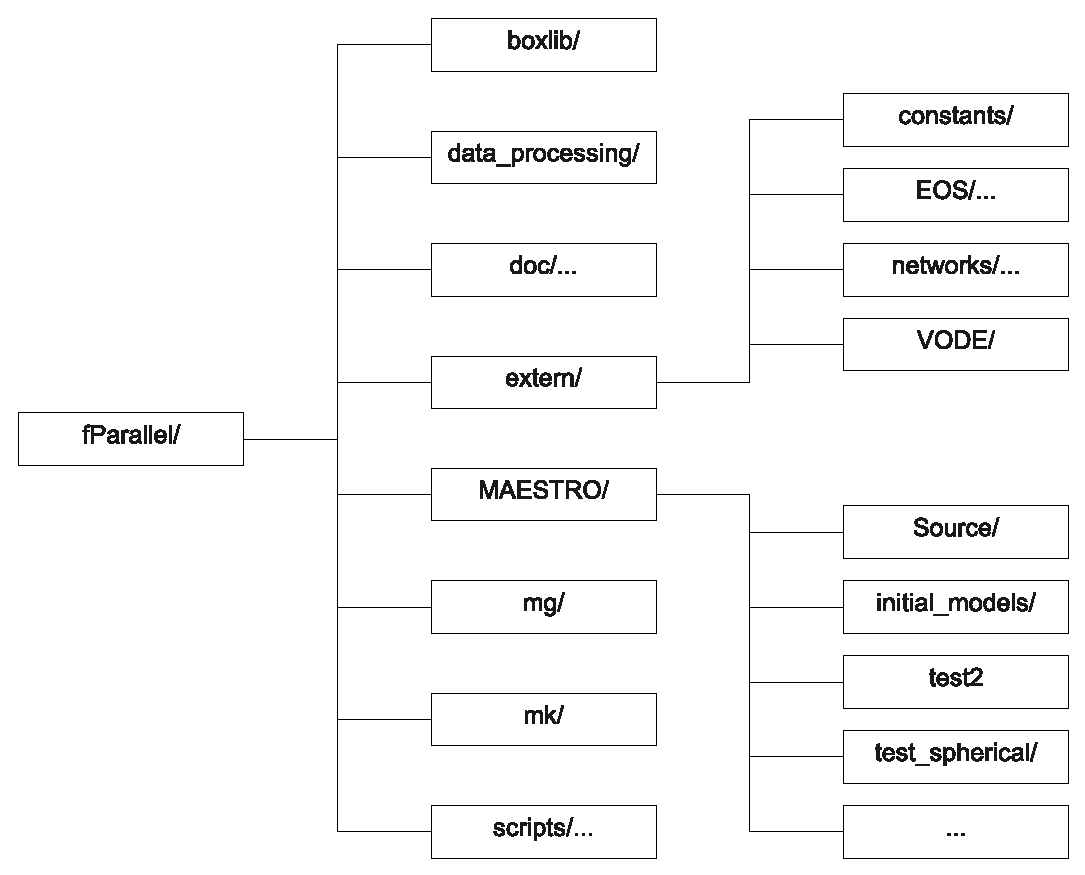
\includegraphics[width=5.0in]{\archfigpath/maestro_directory2}
\caption[MAESTRO directory structure]
{The basic MAESTRO directory structure}
\end{figure}

All the files needed to build MAESTRO are contained in the {\tt
  fParallel} directory structure.  Problems piece together various
MAESTRO directories, choosing a reaction network, equation of state,
and conductivity routine to build an executable.  Briefly, the
sub-directories are:
\begin{itemize}
\item {\tt boxlib/} 

 BoxLib is a library for describing meshes consisting of a union
 of boxes.  The BoxLib modules define the basic datatypes used
 in MAESTRO.  BoxLib also provides the routines that handle the
 parallelization and I/O.

\item {\tt data\_processing/}

 Simple Fortran-based analysis routines (e.g.\ extract a line from a
 multidimensional dataset) that operate on BoxLib datasets.

\item {\tt extern/}

 External modules, like ODE integrators, equations of state, reaction
 networks

 Important subdirectories include:
 \begin{itemize}
 \item {\tt conductivity/}

 Various routines for computing the thermal conductivity used in the
 thermal diffusion part of the algorithm.

 \item {\tt constants/}

 A simple module to define physical constants

 \item {\tt EOS/}

 A collection of various EOSes for use with the code.  The two
 important ones for MAESTRO are {\tt helmeos/} and {\tt
 gamma\_law\_general/}.

 \item {\tt model\_parser/}

 A simple Fortran module for reading in 1-d initial model files.  This
 is used by the initialization routines to get the initial model data.

 \item {\tt networks/}

 Various reaction networks for MAESTRO problems.  In addition to
 providing a routine to evolve the nuclear species due to reactions,
 the networks also define the species that are advected by the code.

 \item {\tt VODE/}

 An integration package for ODEs.  At the moment, this is used 
 for integrating various reaction networks.
 
 \end{itemize}

\item {\tt MAESTRO/}

 The main MAESTRO algorithm directory.  The individual problem directories
 lie under here, and all of the main MAESTRO source lives in the {\tt Source/}
 sub-directory.

 Important directories under {\tt MAESTRO/} include:

 \begin{itemize}

 \item {\tt docs/}

   Documentation describing the basic algorithm (including this
   document).

 \item {\tt initial\_models}

   Several sub-directories containing routines to generate
   1-d initial conditions in hydrostatic equilibrium for 
   mapping onto the MAESTRO grid.  See \S~\ref{sec:initial_models}
   for details.

 \item {\tt Source}

   The main MAESTRO source.  Here you will find the driver routine, the
   advection routines, etc.  All MAESTRO problems will compile this
   source.

 \item problem directories: {\tt test2}, {\tt
   test\_spherical}, $\ldots$

   Each problem in MAESTRO gets it own subdirectory.  The {\tt
     GNUmakefile} in the problem directory includes the instructions
   on how to build the executable, including what modules in {\tt
     extern} are used.

   Any file that you place in a sub-directory here takes 
   precedence over a file of the same name in {\tt MAESTRO/}.
   This allows problems to have custom versions of the main
   MAESTRO routines (e.g.\ initial conditions via {\tt initdata.f90}.
   See \S~\ref{sec:makefile} for details on the build system).

 \end{itemize}

\item {\tt mg/}

  The multigrid solver, with support for both cell-centered and
  node-centered data.

\item {\tt mk/}

  The generic Makefiles that store the compilation flags for
  various platforms.  Platform/compiler-specific options are stored
  in the {\tt comps/} subdirectory.

\item {\tt scripts/}

  Some simple scripts that are useful for building, running,
  maintaining MAESTRO.

\end{itemize}





\section{Getting Started}

In this section we give an overview of MAESTRO, including some of the
standard problems, how to run the code, some basic runtime parameters,
and how to look at the output.


\subsection{`Standard' Test Problems}

Different problems in MAESTRO are contained in individual
sub-directories under {\tt MAESTRO/}.  The {\tt GNUmakefile}
in each problem directory lists the components of {\tt MAESTRO}
that are used to build the executable.  Full details of the
{\tt GNUmakefile} can be found in \S~\ref{sec:adding_problems}.

Some of the test problems available are:
\begin{itemize}
\item {\tt flame} \\[-3mm]

The {\tt flame} problem models a planar laminar flame.  Initially cool
fuel and hot ash are put in pressure equilibrium.  Thermal diffusion
transfers heat to the fuel, driving a burning front.  This problem
does not use the traditional MAESTRO elliptic constraint, but
rather enforces $\nabla \cdot U = S$ (through the runtime parameter
{\tt do\_smallscale = T}) as discussed in \cite{SNe}.

\item {\tt spherical\_heat} \\[-3mm]

{\tt spherical\_heat} maps a spherical star (a Chandrasekhar-mass white
dwarf) onto the Cartesian domain and uses an external heat source to
cause the star to expand.  This is the 3-d analogue of the {\tt
  test\_basestate} unit test (see \S~\ref{sec:unit_tests}).  This
problem was discussed in \cite{multilevel}.

\item {\tt test2} \\[-3mm]

{\tt test2} places 3 hots spots in a plane-parallel atmosphere.
Burning makes these buoyant bubbles which role up.  This problem was
used in \cite{lowMach3} to compare with compressible solvers.

\item {\tt test\_convect} \\[-3mm]

{\tt test\_convect} drives convection through a plane-parallel
atmosphere using an externally-specified heat source.  This problem
was used to compare with compressible solvers in \cite{lowMach3}
and to test the multilevel algorithm in \cite{multilevel}.

\item {\tt test\_spherical} \\[-3mm]

{\tt test\_spherical} sets up an isentropically stratified star
and stirs it up with a random velocity field.  The low Mach number
constraint is replaced with the anelastic constraint (through
the {\tt beta\_type} runtime parameter).  Analytically, under
these conditions, the density of the star should not change.
This test problem was discussed in \cite{lowMach4}.

\end{itemize}


\subsection{Compiling and Running}

To build the MAESTRO executable, simply type `{\tt make}' in the
problem directory.  The executable will have a name like {\tt
  main.Linux.Intel.exe}, where the specific parts of the name depend
on the compilers and OS used.  MAESTRO can be built with support for
parallelism (using MPI or MPI+OpenMP), or compiled as a serial code.
The top portion of the {\tt GNUmakefile} can be editted to choose the
build options.  Setting {\tt MPI := t} will build the code to use MPI
for parallelization.  Setting {\tt OMP := t} will use OpenMP.  OpenMP
is used together with MPI, with MPI distributing the grids across the
processors and within a shared-memory node, OpenMP allows many cores
to operate on the same grid.  A final build option determines whether
to build the code with support for debugging.  Setting {\tt NDEBUG :=
  t} disables debugging features.

If the {\tt helmeos} equation of state is chosen for the problem, then
the data table for the equation of state, {\tt
  extern/EOS/helmeos/helm\_table.dat} needs to be copied to the
directory in which the code is run.

Each problem will have one or more inputs files (for example, {\tt
  test2/inputs\_2d}) which override the default values for one or more
runtime parameters.  The code is run simply as:
\begin{verbatim}
  ./main.Linux.Intel.exe inputs_2d
\end{verbatim}
for a serial executable, and, depending on your MPI environment, something like:
\begin{verbatim}
  mpiexec -n 16 ./main.Linux.Intel.mpi.exe inputs_2d
\end{verbatim}
for the parallel code.

As the code runs, it will output both plotfiles and checkpoints as
well as one of more text diagnostic files (like {\tt
  maestro\_diag.out}) with integral or extrema information (like
maximum Mach number) from each timestep.  By default, the plotfiles
will be named {\tt plt}{\em nnnnn}, where the number {\em nnnnn} is
the timestep number when the file was outputted.  Similarly, the
checkpoints are named {\tt chk}{\em nnnnn}.  BoxLib plotfiles and
checkpoints are actually directories, with the data stored in
subdirectories grouped by refinement level.  Details of the simulation
(build information, number of processors used, output date, output
directory, runtime parameter values, ...) are stored in the {\tt
  job\_info} file in each plotfile directory.

A large number of runtime parameters affect the code's behavior.  Any
runtime parameter can be set either in the inputs file, as {\tt parameter
  = value}, or on the command line by adding {\tt --parameter value} after
listing the inputs file on the command line.  A full list of runtime
parameters is detailed in \S~\ref{sec:runtime_parameters}.  Below we
outline the most common runtime parameters.

\subsection{Controlling Timestepping and Output}

Parameters that set the maximum time for the simulation to run
include:
\begin{itemize}
\item {\tt stop\_time} is the maximum simulation time, in seconds,
      to evolve the system for.

\item {\tt max\_step} is the maximum number of steps to take.
\end{itemize}

\noindent Parameters affecting the size of the timestep include:
\begin{itemize}
\item {\tt cflfac} is a multiplicative factor ({\tt $\le 1$}) 
      applied to the advective CFL timestep

\item {\tt init\_shrink} is the factor ({\tt $\le 1$}) by which to reduce 
      the initial timestep from the estimated first timestep.
\end{itemize}

\noindent Parameters affecting output and restart include:
\begin{itemize}

\item {\tt restart} tells MAESTRO to restart from a checkpoint.  The
      value of this parameter should be the file number to restart from.
      For example, to restart from the checkpoint file {\tt chk00010},
      you would set {\tt restart = 10}.

\item {\tt plot\_int} is the number of steps to take between
  outputting a plotfile

\item {\tt plot\_deltat} is the simulation time to evolve between
  outputting a plotfile.  Note: to output only based on simulation
  time, set {\tt plot\_int = -1}.

\item {\tt check\_int} is the number of steps to take between
  outputting a checkpoint.

\end{itemize}

\subsection{Defining the Grid and Boundary Conditions}

Parameters that determine the spatial extent of the grid, 
the types of boundaries, and the number of computational cells include:
\begin{itemize}

\item {\tt max\_levs } is the maximum number of grid levels in the AMR
  hierarchy to use.  {\tt max\_levs = 1} indicates running with only a
  single level spanning the whole domain.

\item {\tt n\_cellx }, {\tt n\_celly }, {\tt n\_cellz } the size of
  base level in terms of number of cells, in the $x$, $y$, and $z$
  coordinate directions.

\item {\tt max\_grid\_size } the maximum extend of a grid, in any
  coordinate direction, as measured in terms of number of cells.

  For multilevel problems, the parameter {\tt max\_grid\_size\_1}
  controls the maximum extent on level 1 (the base grid), {\tt
    max\_grid\_size\_2} controls the maximum extent on level 2, and
  {\tt max\_grid\_size\_3} controls the maximum extent on levels 3 and
  higher.

\item {\tt prob\_lo\_x }, {\tt prob\_lo\_y }, {\tt prob\_lo\_z } is
  the physical coordinate of the lower extent of the domain boundary
  in the $x$, $y$, and $z$ coordinate directions.

\item {\tt prob\_hi\_x }, {\tt prob\_hi\_y }, {\tt prob\_hi\_z } is
  the physical coordinate of the upper extent of the domain boundary
  in the $x$, $y$, and $z$ coordinate directions.

\item {\tt bcx\_lo }, {\tt bcy\_lo }, {\tt bcz\_lo }, 
      {\tt bcx\_hi }, {\tt bcy\_hi }, {\tt bcz\_hi } are the boundary
   condition types at the lower (`{\tt lo}') and upper (`{\tt hi}')
   domain boundaries in the $x$, $y$, and $z$ coordinate directions.
   The different types are set via integer flags noted below: 

   \begin{center}
   \begin{tabular}{ll}
   \hline
   BC type    & integer flag \\
   \hline
   periodic             & -1 \\
   inlet (user-defined) & 11 \\
   outlet               & 12 \\
   symmetry             & 13 \\
   slip wall            & 14 \\
   no-slip wall         & 15 \\
   \hline
   \end{tabular}
   \end{center}


\end{itemize}

Note that grid cells must be square, i.e. $\Delta x = \Delta y = \Delta z$
where $\Delta x$ on the base grid is computed as $({\tt prob\_hi\_x}
- {\tt prob\_lo\_x})/{\tt n\_cellx}$.  For multilevel problems, the effective
number of zones on the finest grid in the $x$ direction will be
${\tt n\_cellx} \cdot 2^{({\tt max\_levels} -1)}$.



\subsection{Working with the Output}

Visualization and analysis are done with on the plotfiles.  A
number of in-house and externally developed tools can work 
with BoxLib-formatted plotfiles.


\subsubsection{\tt Amrvis}

{\tt Amrvis} is an easy-to-use visualization tool developed at LBL for
2- and 3-d datasets which can plot slices through 3-d datasets as well
as volume-renderings.  It can also very easily extract 1-d lines
through the dataset along any coordinate direction.  It is distributed
separately from the MAESTRO distribution.


\subsubsection{{\tt data\_processing} scripts}

Several useful analysis scripts (written in Fortran 90) can be found
in {\tt fParallel/data\_processing}.  The {\tt GNUmakefile} there
needs to be edited to indicate which of the tools to build.  For
example, to extract the density along a line from the center of a
plotfile, {\tt plt00200}, in the $y$-direction:

\begin{verbatim}
fextract.Linux.gfortran.exe -d 2 -v "density" -p plt00200
\end{verbatim}

These routines are described in \S~\ref{sec:analysis}.




\subsubsection{VisIt}

VisIt is a powerful, DOE-supported visualization tool for 2- and 3-d
datasets.  It can do contouring, volume rendering, streamlines, ...\
directly from BoxLib plotfiles (to open a plotfile in VisIt, point to
the {\tt Header} file inside the plotfile directory).  Details on
visit can be found at {\tt https://wci.llnl.gov/codes/visit/home.html}\,.

\subsubsection{Diagnostic Files}

By default, MAESTRO outputs global diagnostics each timestep into a file
called {\tt maestro\_diag.out}.  This includes the maximum Mach number,
peak temperature, and peak nuclear energy generation rate.  Individual problems
can provide their own {\tt diag.f90} file to produce custom diagnostic
output.


\subsection{Unit Tests}

\label{sec:unit_tests}

In addition to the problems descibed above which use the full
capabilities of MAESTRO, there are a number of unit tests that
exercise only specific components of the MAESTRO solvers.  The
tests have their own drivers (a custom {\tt varden.f90}) that
initialize only the data needed for the specific test and call
specific MAESTRO routines directly.

\begin{itemize}
\item {\tt test\_advect} \\[-3mm]

  This test initializes a Gaussian density field (no other scalar
  quantities are used) and a uniform velocity field in any one of the
  coordinate directions.  The Gaussian profile is advected through
  the period domain exactly once and the error in the density profile
  (L2 norm) is computed.  The driver for this problem does this 
  for every dimension twice (once with a positive velocity and once
  with a negative velocity).  After all coordinate directions are 
  tested, the norms are compared to ensure that the error does
  not show any directional bias.


\item {\tt test\_average} \\[-3mm]

  This test initializes a 1-d radial base state quantity with a
  Gaussian distribution, maps it into the 3-d domain (assuming a
  spherical geometry) using the routines provided by the {\tt
    fill\_3d\_module} module, and then calls {\tt average} to put it
  back onto a 1-d radial array.  This way we test the accuracy of our
  procedure to map between the 1-d radial and 3-d Cartesian states.
  The output from this test was described in detail in
  \cite{multilevel}.

\item {\tt test\_basestate} \\[-3mm]

  This test initializes the base state to contain a hydrostatic
  model and then evolves the state with heating to watch the 
  hydrostatic adjustment of the atmosphere.  In particular,
  the base state velocity, $w_0$, is computed in response to 
  the heating and this is used to advect the base state density
  and compute the new pressure, $p_0$.  An early version of 
  this routine was used for the plane-parallel expansion test
  in \cite{lowMach2}.  This version of the test was also shown
  for a spherical, self-gravitating star in \cite{multilevel}.

  
\item {\tt test\_diffusion}

  This test initializes a Gaussian temperature profile and calls
  the thermal diffusion routines in MAESTRO to evolve the state 
  considering only diffusion.  The driver estimates a timestep
  based on the explicit thermal diffusion timescale and loops
  over calls to the thermal diffusion solver.  A Gaussian remains
  Gaussian when diffusing, so an explicit error can be computed
  by comparing to the analytic solution.  This test is 
  described in \cite{xrb}.


\item {\tt test\_particles}

  This test exercises the particle advection routine.  A simple
  circular velocity field, with the magnitude increasing with radius
  from the center is initialized.  A number of particles are then
  initialized at various radii from the center and they are advected
  for one period.  The particle paths should be perfect circles, and
  the final particle position should overlap with the initial
  position.

  Particle data is stored separately from the fluid data.  Instead
  of being part of the plotfiles, the particle data is outputted
  each timestep into files named {\tt timestamp\_*}, where 
  the number indicates which processor did the writing.  These
  particle files can be processed and the particle data plotted
  using the python routines in {\tt data\_processing/python/}.

\end{itemize}


\section{Adding A New Problem}
\label{sec:adding_problems}

Different MAESTRO problems are defined in subdirectories under
{\tt MAESTRO/}.  To add a problem, start by creating a new
sub-directory---this is where you will compile your problem and
store all the problem-specific files.

The minimum requirement to
define a new problem would be a {\tt GNUmakefile} which describes how
to build the application and an input file which lists the runtime
parameters.  The problem-specific executable is built in the problem
directory by typing {\tt make}.  Source files are found automatically
by searching the directories listed in the {\tt GNUmakefile}.
Customised versions of any source files placed in the problem-directory
override those with the same name found elsewhere.  Any unique
source files (and not simply a custom version of a file found
elsewhere) needs to be listed in a file call {\tt GPackage.mak}
in the problem-directory.

\subsection{The {\tt GNUmakefile}}

\label{sec:makefile}

A basic {\tt GNUmakefile} begins with:
\begin{lstlisting}[language={[gnu]make},mathescape=false]
  NDEBUG := t
  MPI    :=
  OMP    :=
\end{lstlisting}
Here, {\tt NDEBUG} is true if we are building an optimized executable.
Otherwise, the debug version is built---this typically uses less
optimization and adds various runtime checks through compiler flags.
{\tt MPI} and {\tt OMP} are set to true if we want to use either MPI
or OpenMP for parallelization.  If {\tt MPI := t}, you will need to
have the MPI libraries installed, and their location may need to be 
specified in {\tt MAESTRO/mk/GMakeMPI.mak}.

The next line sets the compiler to be used for compilation:
\begin{lstlisting}[language={[gnu]make},mathescape=false]
  COMP := Intel
\end{lstlisting}
The MAESTRO build system knows what options to use for various
compiler families.  The {\tt COMP} flag specifies which compiler to
use.  Allowed values include {\tt Intel}, {\tt gfortran}, {\tt PGI},
and {\tt PathScale}.  The specific details of these choices are
defined in the {\tt MAESTRO/mk/comps/} directory.

{\tt MKVERBOSE} set to true will echo the build commands to the
terminal as the are executed.
\begin{lstlisting}[language={[gnu]make},mathescape=false]
  MKVERBOSE := t
\end{lstlisting}

The next two lines define where the top of the source tree is
include the basic Makefile information (like compiler
flags).
\begin{lstlisting}[language={[gnu]make},mathescape=false]
  FPARALLEL := ../..

  include $(FPARALLEL)/mk/GMakedefs.mak
\end{lstlisting}
%$

A MAESTRO application is built from several packages (the
multigrid solver, an EOS, a reaction network, etc.).  The core
MAESTRO packages are always included, so a problem only needs
to define the EOS, reaction network, and conductivities to
use, as well as any extra, problem-specific files.  
\begin{lstlisting}[language={[gnu]make},mathescape=false]
EOS_DIR := extern/EOS/helmeos   
CONDUCTIVITY_DIR := extern/conductivity/constant
NETWORK_DIR := extern/networks/ignition

EXTRA_DIR := extern/random
\end{lstlisting}
Generally, one does not need to include the problem directory itself
in {\tt EXTRA\_DIR}, unless there are unique source files found there,
described in a {\tt GPackage.mak} file.  These variables are
interpreted by the {\tt GMaestro.mak} file and used to build a master
list of packages called {\tt Fmdirs}.  The build system will attempt
to build all of the files listed in the various {\tt GPackage.mak}
files found in the {\tt Fmdirs} directories.  Furthermore, {\tt
  Fmdirs} will be will be added to the {\tt make} {\tt VPATH}, which
is the list of directories to search for source files.  The problem
directory will always be put first in the {\tt VPATH}, so any source
files placed there override those with the same name found elsewhere
in the source tree.  

Some packages (for instance, the {\tt helmeos}
EOS) require Fortran include files.  The {\tt Fmincludes} variable
lists all those directories that contain include files that are
inserted into the Fortran source at compile time via the {\tt include}
statement.  Presently, the only instance of this is with the Helmholtz
general equation of state found in {\tt extern/EOS/helmeos/}.  This is
automatically handled by the {\tt GMaestro.mak} instructions.

Runtime parameters listed in the {\tt MAESTRO/\_parameters} file are
parsed at compile time and the file {\tt probin.f90} is written and
compiled.  This is a Fortran module that holds the values of the
runtime parameters and makes them available to any routine.  The
variable {\tt PROBIN\_PARAMETERS} should list all of the files that
contain runtime parameters for the current problem.  You must always
include the main {\tt ../\_parameters} file (i.e.\ {\tt
  MAESTRO/\_parameters}).  Sometimes a problem defines their own
runtime parameters (for instance {\tt \_parameters.myproblem}), in which
case, its parameter file should also appear in {\tt
  PROBIN\_PARAMETERS} (see \S~\ref{sec:def_runtime_param}).
\begin{lstlisting}[language={[gnu]make},mathescape=false]
  PROBIN_PARAMETERS := ../_parameters
\end{lstlisting}

The final line in the {\tt GNUmakefile} includes the rules to actually
build the executable.
\begin{lstlisting}[language={[gnu]make},mathescape=false]
  include $(FPARALLEL)/MAESTRO/GMaestro.mak
\end{lstlisting}
%$


\subsubsection{Handling Problem-Specific Source Files}

As mentioned above, any source files placed in the problem directory
override a files with the same name found elsewhere in the source
tree.  This allows you to create a problem-specific version of any
routine.  Source files that are unique to this problem (i.e.\ there is
no file with the same name elsewhere in the source tree) need to be
listed in a file {\tt GPackage.mak} in the problem directory, and
the problem-directory needs to be explicitly listed in the {\tt EXTRA\_DIR}
list in the {\tt GNUmakefile}.


\subsection{Defining Runtime Parameters}

\label{sec:def_runtime_param}

The runtime parameters for the core MAESTRO algorithm are listed
in {\tt MAESTRO/\_parameters}.  That file is parsed at compile-time
by the {\tt MAESTRO/write\_probin.py} script
(along with any other parameter files listed in the {\tt PROBIN\_PARAMETERS}
variable in the {GNUmakefile}, see \S \ref{sec:makefile}).  The script
outputs the {\tt probin.f90} source file.  Each line
in the {\tt \_parameters} file has the form: 
\vskip 3mm
{\em parameter} \hskip 10em  {\em data-type} \hskip 10em  {\em value} 
\vskip 3mm
\noindent where {\em parameter} is the name of the runtime parameter,
{\em data-type} is one of \{{\tt character}, {\tt real}, {\tt
  integer}, {\tt logical}\}, and the {\em value} specifies the default
value for the runtime parameter.  Comments are indicated by a `{\tt
  \#}' character and a used to produce documentation about the
available runtime parameters.

At runtime, the default values for the parameters can be overridden
either through the inputs file (by adding a line of the form: {\tt
  parameter = value}) or through a command-line argument (taking the
form: {\tt --parameter value}).  The {\tt probin\_module} makes the
values of the runtime parameters available to the various functions
in the code (see \S~\ref{sec:probin}).

Problem-specify runtime parameters should be defined in the
problem-directory in a file called {\tt
  \_parameters}\{{\em.problem-name}\}.  This file should be added
to the {\tt PROBIN\_PARAMETERS} variable in the {\tt GNUmakefile}.



\subsection{Preparing the Initial Model}

\label{sec:initial_models}

MAESTRO models subsonic flows that are in hydrostatic equilibrium.
The solution in MAESTRO is broken up into a 1-d base state and the 2-
or 3-d full state.  The job of the 1-d base state in the algorithm is
to represent the hydrostatic structure.  The full, Cartesian state
carries the departures from hydrostatic equilibrium.  The underlying
formulation of the low Mach number equations assumes that the base
state is in hydrostatic equilibrium.  At the start of a simulation,
the initial model is read in and taken as the base state.  Therefore,
any initial model needs to already be in hydrostatic equilibrium.

The routines in {\tt MAESTRO/initial\_model/} prepare an initial model
for MAESTRO.  There are two types of routines here, the first type
take an existing 1-d initial model produced somewhere else (e.g.\ a
1-d stellar evolution code), and and map it onto a uniform grid, at
the desired resolution, using the equation of state in MAESTRO, and
using MAESTRO's discretization of hydrostatic equilibrium.  The second
type generate the initial model internally, by integrating the
condition of hydrostatic equilibrium together with a simplifying
assumption on the energy (e.g. isothermal or isentropic).  In
both cases hydrostatic equilibrium is enforced as:
\begin{equation}
\frac{p_{i+1} - p_i}{\Delta r} = \frac{1}{2} (\rho_i + \rho_{i+1})
g_{i+1/2}
\end{equation}
Here, $g_{i+1/2}$ is the edge-centered gravitational acceleration.

The {\tt toy\_atm} example provides a simple approximation for a thin
(plane-parallel) convectively-unstable accreted layer on the surface
of a star.  This can be used as the starting point for a more complex
model.  

MAESTRO initial models are read in by the {\tt extern/model\_parser}
routines.  This expects the initial model to contain a header giving
the number of variables and their names, followed by rows of data
giving the coordinate and data values at that coordinate.  The initial
model should contain the same species data (as mass fractions) as
defined in the {\tt network} module used by the MAESTRO problem.

Full details on which initial model routine matches each problem and
how the initial models are used to initialize the full state data can
be found in \S~\ref{sec:initial_models_main}.



\section{BoxLib Data Structures}

\begin{figure}[t]
\centering
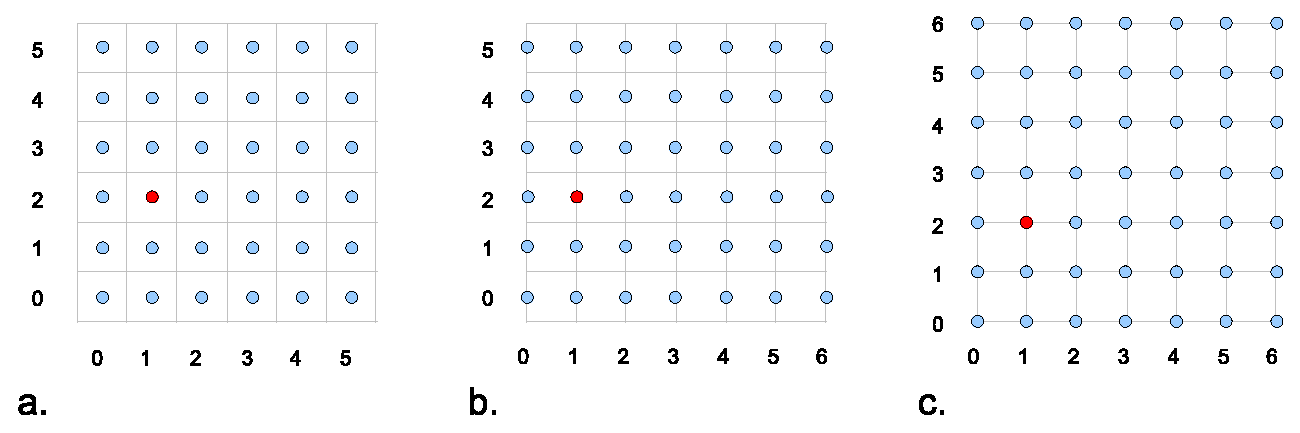
\includegraphics[width=6.5in]{\archfigpath/data_loc2}
\caption[Data-centerings on the grid]
  {\label{fig:dataloc} Some of the different data-centerings:
  (a) cell-centered, (b) nodal in the $x$-direction, and (c) nodal in
  both the $x$- and $y$-directions.  Note that for nodal data, the
  integer index corresponds to the lower boundary in that direction.
  In each of these centerings, the red point has the same indices:\ (1,2).
  Not shown is the case where data is nodal in the $y$-direction only.}
\end{figure}

MAESTRO's gridding is handled by the BoxLib library.  The underlying
idea in BoxLib is to allow for adaptive mesh refinement (AMR)---different
regions of the domain can have different spatial resolutions.  The
domain is broken into boxes.  At the coarsest (base) level of
refinement, the entire computational domain is covered, either by one
box or broken across many boxes.  Higher levels of refinement have
finer zones (typically $2\times$).  Only a portion of the domain may
be covered by the higher levels of refinement.  

\MarginPar{Nesting? ghost cells?}
For parallel computations, the boxes are spread across processors, in
a fashion designed to put roughly equal amounts of work on each
processor (load balancing).

On a grid, the data can be stored at cell-centers, on a face/edge, or
on the corners.  In BoxLib, data that is on an edge is termed `nodal'
in that direction (see Figure~\ref{fig:dataloc}).  Data that is on the
corners is nodal in all spatial directions.  In MAESTRO, the state
data (density, enthalpy, velocity, $\ldots$) is generally
cell-centered.  Fluxes are nodal in the direction they represent.
A few quantities are nodal in all directions (e.g.\ $\phi$ used in
the final velocity projection).

To simplify the description of the underlying AMR grid, BoxLib
provides a number of Fortran types.  We briefly summarize the major
data types below.


\subsection{\boxtype}

A \boxtype\ is simply a rectangular domain in space.  Note that boxes
do not hold the state data themselves.  A \boxtype\ has a {\tt lo} 
and {\tt hi} index in each coordinate direction that gives the
location of the lower-left and upper-right corner with respect to
a global index space.  

\begin{figure}[t]
\centering
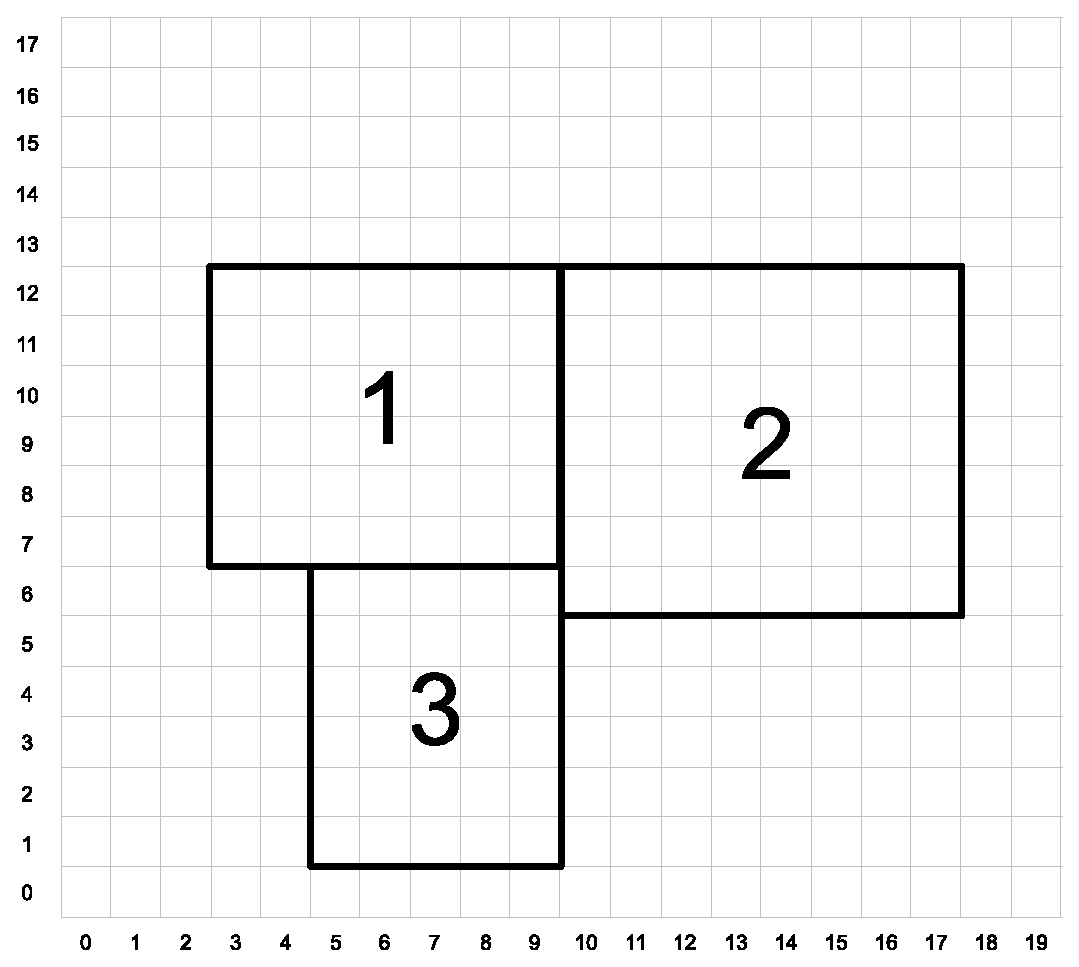
\includegraphics[width=4.0in]{\archfigpath/index_grid2}
\caption[Single-level grid structure]
{\label{fig:boxes} Three boxes that comprise a single level.  At this
  resolution, the domain is 20$\times$18 zones.  Note that the
  indexing in BoxLib starts with $0$.}
\end{figure}


The computational domain is divided into boxes.  The collection of
boxes with the same resolution comprise a level.
Figure~\ref{fig:boxes} shows three boxes in the same level of
refinement.  The position of the boxes is with respect to the global
index space at that level.  For example, box 1 in the figure has {\tt
  lo} = (3,7) and {\tt hi} = (9,12).  Note that the global indexing
is 0-based.

The global index space covers the entire domain at a given resolution.
For a simulation setup with {\tt n\_cellx = 32} and {\tt n\_celly =
  32}, the coarsest level (level 1) has $32 \times 32$ zones, and the
global index space will run from $0, \ldots, 31$ in each coordinate
direction.  Level 2 will have a global index space running from $0,
\ldots, 63$ in each coordinate direction (corresponding to $64 \times
64$ zones if fully refined), and level 3 will have a global index
space running from $0, \ldots, 127$ in each coordinate direction
(corresponding to $128\times 128$ zones if fully refined).


\subsubsection{Common Operations on a \boxtype}

A \boxtype\ declared as:
\begin{verbatim}
  type(box) :: mybox
\end{verbatim}
%
The upper and lower bounds of the box (in terms of the global
index space) are found via:
\begin{itemize}

\item {\tt lo = lwb(mybox)} returns an array, {\tt lo(dm)}, with
     the box lower bounds

\item {\tt hi = upb(mybox)} returns an array, {\tt hi(dm)}, with
     the box upper bounds

\end{itemize}




\subsection{\boxarray\ and \mlboxarray}

A \boxarray\ is an array of boxes.  A \mlboxarray\ is a collection of
\boxarray s at different levels of refinement.

\subsection{\layout\ and \mllayout}

A \layout\ is basically a \boxarray\ that knows information about other
boxes, or box ``connectivity.''  It contains additional information
that is used in filling ghost cells from other fine grids or from
coarser grids.  This information is stored as long as the layout
exists so that we don't have to recompute intersections every time we
do some operation with two multifabs that have that layout, for
example.


\subsection{\fab}

A \fab\ is a ``Fortran Array Box''.  It contains the state data in a
multidimensional array and several \boxtype-types to describe where in
the global index-space it lives.  
Note that all state data is stored in a four-dimensional array,
{\tt (nx,ny,nz,nc)} in size, regardless of the dimensionality of the
problem.  Here {\tt nc} is the number of components, for instance
representing different fluid variables.  For 2D problems, {\tt nz=1}.

A \fab\ would represent the data for a single box in the domain.
In MAESTRO, we don't usually deal with \fab s alone, but rather
we deal with \multifab s, described next.

\subsection{\multifab}

A \multifab\ is a collection of \fab s at the same level of
refinement.  This is the primary data structure that MAESTRO
routine operate on.  A multilevel simulation stores the 
data in an array of multifabs, where the array index refers
to the refinement level.

\subsubsection{Working with \multifab s}

To build a \multifab, we need to provide a \layout, the number of
components to store in the multifab, and the number of ghostcells.  In
MAESTRO, the hierarchry of grids will be described by a single
\mllayout.  A \multifab\ can be declared and built at any time in a
simulation using the \mllayout, thereby allocating space at every
grid location in the simulation.  The sequence to build a \multifab\
appears as
\begin{lstlisting}[language={[95]fortran},mathescape=false]
  type(multifab) :: mfab(nlevs)
  ...
  do n = 1, nlevs
     call multifab_build(mfab(n), mla%la(n), nc, ng)
  enddo
\end{lstlisting}
Here, {\tt nc} is the number of components and {\tt ng} is the number
of ghostcells.  The \multifab\ is built one level at a time, using the
\layout\ for that level taken from the \mllayout, {\tt mla}.

A common operation on a \multifab\ is to initialize it to $0$
everywhere.  This can be done (level-by-level) as
\begin{lstlisting}[language={[95]fortran},mathescape=false]
call setval(mfab(n), ZERO, all=.true.)
\end{lstlisting}
where {\tt ZERO} is the constant 0.0 from {\tt bl\_constants\_module}.

The procedure for accessing the data in each grid managed by the \multifab\
is shown in \S~\ref{sec:example}.  
Subroutines to add, multiply, or divide two \multifab s exist, as do
subroutines to copy from one \multifab\ to another---see {\tt boxlib/multifab.f90}
for the full list of routines that work with \multifab s.


When you are done working with a \multifab, its memory can be freed by
calling {\tt multifab\_destroy} on the \multifab.




\subsection{\bctower}

A \bctower\ holds the information about what boundary conditions are
in effect for each variable in a MAESTRO simulation.  \MarginPar{better description?}

\section{MAESTRO Data Organization}

The state of the star in MAESTRO is described by both a
multidimensional state and the 1D base state.  The full
multidimensional state is stored in \multifab s while the base state
is simply stored in Fortran arrays.  Here we describe the
major MAESTRO data-structures.




\subsection{`{\tt s}' \multifab s (fluid state)}

The fluid state (density, enthalpy, species) are stored together in a
cell-centered multi-component \multifab, typically named {\tt sold},
{\tt s1}, {\tt s2}, or {\tt snew} (depending on which time-level it
represents).  The enthalpy is stored as $(\rho h)$, and the species
are stored as partial-densities $(\rho X_k)$.

Individual state variables should be indexed using the integer keys provided 
by the {\tt variables} module (see \S \ref{sec:variables_module}).  For example,
the integer {\tt rho\_comp} will always refer to the density component of the state.


\subsection{`{\tt u}' \multifab s (fluid velocity)}

The fluid velocity at time-levels $n$ and $n+1$ is stored in
a cell-centered multi-component \multifab, typically named
{\tt uold} or {\tt unew}.  Here the {\tt dm}
components correspond to each coordinate direction.

\subsection{{\tt umac} (the MAC velocity)}

In creating the advective fluxes, we need the time-centered velocity
through the faces of the zone---the $x$-velocity on the $x$-edges, the
$y$-velocity on the $y$-edges, etc.\ (see figure~\ref{fig:mac}).  This
type of velocity discretization is termed the MAC velocity (after the
``marker-and-cell'' method for free boundaries in incompressible
flows \cite{harlowwelch:1965}).



\begin{figure}[t]
\centering
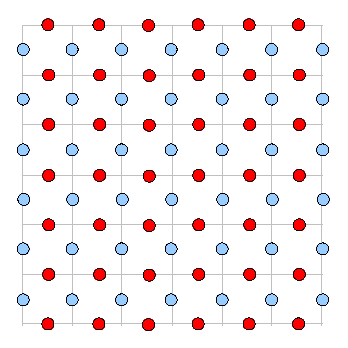
\includegraphics[width=2.5in]{\archfigpath/mac2}
\hspace{0.1in}
\begin{minipage}[b]{3.8in}
\caption[The MAC grid]
{\label{fig:mac} The MAC grid for the velocity.  
Here the $x$-velocity is on the $x$-edges (shown as the 
blue points) and the $y$-velocity is on the $y$-edges
(shown as the red points).
}\ \\
\end{minipage}
\end{figure}

The MAC velocities are allocated at each level of refinement, {\tt n},
by making a \multifab\ array where each of the {\tt dm} components is
nodal in its respective direction:
\begin{lstlisting}[language={[95]fortran},mathescape=false]
  type(multifab) :: umac(dm)

  do comp=1,dm
     call multifab_build_edge(umac(n,comp), mla%la(n),1,1,comp)
  enddo
\end{lstlisting}



\subsection{Base State Arrays}

The base state is defined by $\rho_0$, $p_0$, and $w_0$.  There is no
base state composition.  Other arrays are defined as needed, such as
$h_0$, the base state enthalpy.

The base state arrays are 2-dimensional, with the first dimension
giving the level in the AMR hierarchy and the second the radial index
into the base state.  For spherical geometries, the base state only
exists at a single level, so the first index will always be 1.  The
radial index is 0-based, to be consistent with the indexing for the
Cartesian state data.  For example, the base state density would be
dimensioned: {\tt rho0(nlevs,0:nr\_fine-1)}.  Here, {\tt nlevs} is the
number of levels of refinement and {\tt nr\_fine} is the number of
cells in the radial direction at the finest level of refinement.

For multilevel, plane-parallel geometry, all grids at the same height
will have the same resolution so that the full state data is always
aligned with the base state (see Figure~\ref{fig:base_state}).  Base
state data on coarse grids that are covered by fine grids is not
guaranteed to be valid.

For spherical problems, the base state resolution, $\Delta r$, is
generally picked to be finer than the Cartesian grid resolution,
$\Delta x$, i.e.\ $\Delta r < \Delta x$.  The ratio is controlled
by the parameter {\tt drdxfac}.



\section{MAESTRO Helper Modules}

A number of MAESTRO modules appear frequently throughout the source.
Below, we describe some of the more common functionality of the most
popular modules.

\subsection{\tt average}

The {\tt average} module provides a routine {\tt average} that takes
a multilevel \multifab\ array and averages the full Cartesian data
onto the 1-d base state.

\subsection{{\tt eos\_module}}

The {\tt eos\_module} provides the interface to the equation of 
state to connect the state variables thermodynamically.  It 
gets the information about the fluid species from the {\tt network}
module (for example, the atomic number, $Z$, and atomic weight, $A$,
of the nuclei).

Presently there are 2 equations of state that work with MAESTRO:
\begin{itemize}
\item {\tt extern/EOS/helmeos/} represents a general stellar equation 
      of state, consisting of nuclei (as an ideal gas), radiation,
      and electrons (with arbitrary degeneracy and degree of relativity).
      This equation of state is that described in \cite{timmes_eos}.

\item {\tt extern/EOS/gamma\_law\_general} assumes an ideal gas with a mixed 
     composition and a constant ratio of specific heats, $\gamma$:
      \begin{equation}
      p = \rho e (\gamma - 1) = \frac{\rho k_B T}{\mu m_p} 
      \end{equation}
     where $k_B$ is Boltzmann's constant and $m_p$ is the mass of the
     proton.
     The mean molecular weight, $\mu$, is computed assuming 
     electrically neutral atoms:
     \begin{equation}
     \mu = \left ( \sum_k \frac{X_k}{A_k} \right )^{-1}
     \end{equation}
     An option in the source code itself exists for treating the
     species as fully-ionized, but there is no runtime-parameter to
     make this switch.
\end{itemize}

The {\tt eos\_module} declares for convenience the variables that need
appear in the {\tt eos} call argument list.  MAESTRO routines use
these module variables in the EOS call to avoid having to declare 
each quantity in each routine that calls the EOS.

The first argument to the {\tt eos} call is an integer key that
specifies which thermodynamic variables (in addition to the mass
fractions) are used as input.  Options include:

   \begin{center}
   \begin{tabular}{lc}
   \hline
   key            & input quantities \\
   \hline
   eos\_input\_rt       & $\rho$, $T$ \\
   eos\_input\_rh       & $\rho$, $h$ \\
   eos\_input\_tp       & $T$, $p$ \\
   eos\_input\_rp       & $\rho$, $p$ \\
   eos\_input\_re       & $\rho$, $e$ \\
   eos\_input\_ps       & $p$, $s$ \\
   \hline
   \end{tabular}
   \end{center}




\subsection{{\tt fill\_3d\_module}}

The {\tt fill\_3d\_module} provides routines that map from the 1-d
base state to the full Cartesian 2- or 3-d state.  Variations in the
routines allow for cell-centered or edge-centered data on either the
base state or full Cartesian state.

\subsection{{\tt geometry}}

\subsection{{\tt network}}

The {\tt network} module defines the number species advected by the
code ({\tt nspec}), their ordering, and gives their basic properties
(like atomic number, $Z$, and atomic mass, $A$).  All MAESTRO problems
require a {\tt network} module, even if there are no reactions
modeled.  Many different reaction modules (containing different sets
of isotopes) exist in {\tt extern/networks}.  The particular network
used by a problem is defined in the problem's {\tt GNUmakefile}.

To find the location of a particular species (for instance, ``carbon-12'')
in the allowed range of {\tt 1:nspec}, you do the following query:
\begin{lstlisting}[language={[95]fortran},mathescape=false]
  ic12 = network_species_index("carbon-12")
\end{lstlisting}
If the resulting index is {\tt -1}, then the requested species was not
found.

\subsection{{\tt probin\_module}}

\label{sec:probin}

{\tt probin\_module} provides access to the runtime parameters.
The runtime parameters appear simply as module variables.  To get the 
value of a parameter, one simply needs to `{\tt use probin\_module}'.
The preferred method is to add the `{\tt only}' clause to the
{\tt use} statement and explicitly list only those parameters that
are used in the routine.  Defining new runtime parameters is
described in \S~\ref{sec:def_runtime_param}.

\subsection{{\tt variables}}

\label{sec:variables_module}

The {\tt variables} module provides integer keys to index the state
multifabs and other arrays dealing with the scalar quantities.  The
most commonly used keys are are:

\begin{center}
\begin{tabular}{ll}
\hline
{\tt rho\_comp}  & density \\
{\tt rhoh\_comp} & density $\times$ specific enthalpy, $(\rho h)$ \\
{\tt spec\_comp} & first species partial density, $(\rho X_1)$ \\
{\tt temp\_comp} & temperature \\
\hline
\end{tabular}
\end{center}

The species indices are contiguous in the state array, spanning {\tt spec\_comp:spec\_comp-1+nspec}.
To find a particular species, a query can be made through the {\tt
  network} module, such as:
\begin{verbatim}
  ic12 = network_species_index("carbon-12")
\end{verbatim}
and then the \fab\ can be indexed using {\tt spec\_comp-1+ic12} to
get ``carbon-12''.
The {\tt variables} module also provides keys for the plotfile
variables and boundary condition types.


\section{BoxLib Helper Modules}

There are a large number of modules in {\tt boxlib/} that provide
the core functionality for managing grids.  Here we describe
the most popular such modules.


\subsection{{\tt bl\_types}}

\subsection{{\tt bl\_constants}}

\subsection{{\tt parallel}}

\section{\label{sec:example} Example: Accessing State Data}

In MAESTRO, the state data is stored in a multifab array (the array
index refers to the AMR level).  A typical way to extract the state data
array looks like:

\begin{lstlisting}[language={[95]fortran},mathescape=false]
  subroutine example(s,dx,dt)

    use bl_types
    use multifab_module
    use geometry, only: dm, nlevs
    use variables, only: rho_comp
\end{lstlisting}

\noindent Here, the {\tt bl\_types} and {\tt multifab\_module} modules
bring in the basic BoxLib data types. Specifically, here, {\tt
bl\_types} defines {\tt dp\_t} which is the {\tt kind} used for
declaring double precision data, and {\tt multifab\_module} defines
the \multifab\ data type.  The {\tt geometry} module is a MAESTRO
module that provides the dimensionality ({\tt dm}) and the number of 
levels ({\tt nlevs}).  The {\tt variables} module is a MAESTRO
module that provides integer keys for indexing the state arrays.  In
this case the integer {\tt rho\_comp} refers to the location in the
state array corresponding to density.

\begin{lstlisting}[language={[95]fortran},mathescape=false]
    type(multifab) , intent(inout) :: s(:)
    real(kind=dp_t), intent(in   ) :: dx(:,:),dt
\end{lstlisting}

\noindent Next we declare the subroutine arguments.  Here, {\tt s(:)}
is our \multifab\ array that holds the state data.  The array index
in {\tt s} refers to the AMR level.

\begin{lstlisting}[language={[95]fortran},mathescape=false]
    ! Local variables
    real(kind=dp_t), pointer :: sp(:,:,:,:)
    integer :: i,n,ng_sp
    integer :: lo(dm),hi(dm)
\end{lstlisting}

\noindent Amongst the local variables we define here are a pointer,
{\tt sp}, that will point to a single \fab\ from the
\multifab\ {\tt s}.

\begin{lstlisting}[language={[95]fortran},mathescape=false]
    ng_sp = nghost(s(1))
\end{lstlisting}

\noindent Here we get the number of ghostcells for this particular
\multifab.  This will be needed to access the data stored in the
\fab s.  Note that all levels in a \multifab\ will have the same
number of ghostcells, so we can use {\tt s(1)} here.

\begin{lstlisting}[language={[95]fortran},mathescape=false]
    do n=1,nlevs
       do i = 1, s(n)%nboxes
\end{lstlisting}

\noindent To access the data, we loop over all the levels, and
all the boxes in the given level.  {\tt s(n)\%nboxes} is simply
the number of boxes in level {\tt n}.

\begin{lstlisting}[language={[95]fortran},mathescape=false]
          if ( multifab_remote(s(n), i) ) cycle
          sp => dataptr(s(n), i)
          lo =  lwb(get_box(s(n), i))
          hi =  upb(get_box(s(n), i))
\end{lstlisting}

\noindent For parallel runs, there is no guarantee that the particular
box is on the current processor.  The function {\tt multifab\_remote}
returns {\tt .true.} if the box is off-processor, in which case, we 
simply skip to the next box.

The actual data array is accessed through the {\tt dataptr} function,
which takes a \multifab\ (in this case, {\tt s(n)}) and the index of
the \boxtype\ ({\tt i}) we want.  {\tt sp} is always four-dimensional:
3 spatial dimensions and 1 for the components.

Finally, the index bounds of the box (just the data, not the ghostcells) are 
stored in the {\tt dm}-dimensional arrays {\tt lo} and {\tt hi}

\begin{lstlisting}[language={[95]fortran},mathescape=false]
          select case (dm)
          case (2)
             call example_2d(sp(:,:,1,rho_comp),ng_sp,lo,hi,dx(n,:),dt)
          case (3)
             call example_3d(sp(:,:,:,rho_comp),ng_sp,lo,hi,dx(n,:),dt)
          end select
       enddo    ! end loop over boxes

    enddo    ! end loop over levels

  end subroutine example
\end{lstlisting}

\noindent Finally, in this example, we call either the function
{\tt example\_2d} for two-dimensional data or {\tt example\_3d}
for three-dimensional data.  Note that in the two-dimensional
case, we index the data as {\tt sp(:,:,1,rho\_comp)}.  Here a
`{\tt 1}' is used as the `z'-coordinate spatial index, since this
is a 2D problem, and the density component of the state is selected
(using the integer key {\tt rho\_comp}).

This routine will be supplimented with {\tt example\_2d} and {\tt
example\_3d}, which actually operate on the data.  The form of 
these functions is:

\begin{lstlisting}[language={[95]fortran},mathescape=false]
  subroutine example_2d(density,ng_sp,lo,hi,dx,dt)

    use bl_constants_module
    use probin_module, only: prob_lo

    integer        , intent(in) :: lo(:),hi(:), ng_sp
    real(kind=dp_t), intent(in) :: density(lo(1)-ng_sp:,lo(2)-ng_sp:)
    real(kind=dp_t), intent(in) :: dx(:),dt

    integer         :: i, j
    real(kind=dp_t) :: x, y

    do j = lo(2), hi(2)
       y = prob_lo(2) + (dble(j) + HALF)*dx(2)

       do i = lo(1), hi(1)
          x = prob_lo(1) + (dble(i) + HALF)*dx(1)

          ! operate on density(i,j)
          ! ...

       enddo
    enddo

  end subroutine example_2d
\end{lstlisting}

\noindent In this function, the bounds of the {\tt density} array
take into account the {\tt ng\_sp} ghostcells.  The {\tt j} and {\tt i}
loops loop over all the valid zones.  Coordinate information is 
computed from {\tt dx} and {\tt prob\_lo} which is the physical
lower bound of the domain.  {\tt bl\_constants\_module} declares
useful double-precision constants, like {\tt HALF} (0.5).

The three-dimensional case is similar, with the {\tt density} array
declared as 
\begin{lstlisting}[language={[95]fortran},mathescape=false]
  density(lo(1)-ng_sp:,lo(2)-ng_sp:,lo(3)-ng_sp:)
\end{lstlisting}
and an additional loop over the `z' coordinate (from {\tt lo(3)} to
{\tt hi(3)}).



\section{Filling Ghostcells}

Ghostcells are filled through a variety of different routines, depending
on the objective.

\begin{itemize}

\item {\tt multifab\_fill\_boundary} fills ghost cells for two
  adjacent grids at the same level, which als includes periodic domain
  boundary ghost cells.

\item {\tt multifab\_physbc} fills ghostcells at the physical boundaries.

\item {\tt multifab\_fill\_ghost\_cells} is used for multilevel
  problems, and fills ghostcells in the finer grid (level {\tt n}) by
  interpolating from data in the coarser grid (level {\tt n-1}).
  This function, by default, will also call {\tt multifab\_fill\_boundary}
  and {\tt multifab\_physbc} for both levels {\tt n} and {\tt n-1} (you 
  can override this behavior for speed optimization purposes).
  This call is usually preceded by a call to 
  {\tt ml\_cc\_restriction\_c} which sets the level {\tt n-1} data to be
  the average of the level {\tt n} data covering it.
   

\end{itemize}

\section{Boundary Conditions}


\section{Multigrid}

MAESTRO uses the multigrid solver to enforce the divergence constraint
both on the half-time edge-centered advective velocities (the ``MAC
projection'') and on the final cell-centered velocities (the ``HG
projection'').  For the MAC projection, since the velocity data is
edge-centered (the MAC grid), the projection is cell-centered.  For
the HG projection, since the velocity data is cell-centered, the
projection is node-centered.  \MarginPar{should draw a figure} The multigrid solver performs a number
of V-cycles until the residual drops by 10-12 orders-of-magnitude.
There are several options that affect how the multigrid solver
behaves, which we describe below.

\subsection{Special Bottom Solver}
We have a special bottom solver type that greatly speeds up large problems
and speeds up smaller problems to a lesser degree.
In fact, you should use this bottom solver whenever possible, because I
have yet to find a case that performs worse than our standard bottom solver.
What this special solver essentially does is take the data from the coarsest 
level of the original multigrid V-cycle and copy it onto a new grid structure 
with the same number of total cells in each direction, but with a fewer number of larger 
grids.  A new V-cycle begins from this point, 
so we are essentially coarsening this ``new'' problem.
Now, the coarsest level of the multigrid V-cycle in the ``new'' problem has 
fewer cells and fewer grids as compared to the original coarsest level.

To enable this solver, set {\tt hg\_bottom\_solver = 4} (for the nodal
projections) and/or {\tt mg\_bottom\_solver = 4} (for the cell-centered
projections) in your inputs file.

To understand how this bottom solver works, the first thing you need to know
is what the grid structure of the coarsest level of your multigrid V-cycle
looks like (we need to put a description of this in the section above).
Now, figure out the size of the box you would need if you
wanted it to fit all the data on the coarsest level.  Now, figure out what
the largest integer $n$ is so that you can evenly divide the length of this box
by $2^n$ in every coordinate direction.  If $n < 2$, the program will abort
since the grid structure is not suitable for this bottom solver.

Now the code will set up a ``new'' problem, using the data at the coarsest level
of the original problem as the initial data.  The grid structure for this new
problem has the same number of cells as the coarsest level of the original problem,
but the data is copied onto a grid structure where each grid has $2^n$ cells
on each side.  The new V-cycle continues down to the new coarsest level, in
which each grid has 2 cells on each side.  If you wish to impose a limit on
the maximum value that $n$ can have, you can do so by setting 
{\tt max\_mg\_bottom\_nlevs} equal to that value.

{\bf Example 1:} A 3D problem with $384^3$ cells divided into $32^3$ grids, i.e., 
there is a $12\times 12\times 12$ block of $32^3$ grids.  The coarsest level of the 
multigrid V-cycle contains $12\times 12\times 12$ grids that have $2^3$ cells, so the 
entire problem domain has $24^3$ cells.  We see that $n=3$, and create a new problem 
domain with a $3\times 3\times 3$ block of $8^3$ grids.  The coarsest level of the 
multigrid V-cycle for the ``new'' problem will be a $3\times 3\times 3$ block of 
$2^3$ grids.

{\bf Example 2:} A 2D problem with $96\times 384$ cells divided into $48^2$ grids, i.e., 
there is a $2\times 8$ block of $48^2$ grids.  The coarsest level of the multigrid 
V-cycle contains $2\times 8$ grids that have $3^2$ cells, so the entire problem 
domain has $6\times 24$ cells.  We see that $n=1$, so the program aborts since this grid
structure is not appropriate for the fancy bottom solver.


\section{Multilevel and Refinement Criteria}


\section{Particles}

MAESTRO has support for Lagrangian particles that are passively
advected with the velocity field.  These are useful for diagnostics
and post-processing.  To use particles, particles must be seeded into
the domain by writing a problem-specific {\tt init\_particles.f90}
routine.  This routine is called at the start of the simulation.  The
{\tt init\_particles} routines add particles at specific locations by
calling the {\tt particle\_module}'s {\tt add} routine when a given
criteria is met by the fluid state.

When you run the code, particles are enabled by setting {\tt
  use\_particles = T}.  At the end of each timestep the locations of
all the particles are written out into a series of files called {\tt
  timestamp\_NN}, where {\tt NN} is the CPU number on which the
particle {\em currently} resides.  Particles are always kept on the
processor containing the state data corresponding to their present
location.  Several bits of associated data (density, temperature, and
mass fractions) are stored along with the particle ID and position.

Some simple python scripts allow for the plotting of the particle
positions.  For example, running {\tt test2} with particles enabled
will seed particles in the initial hotspot.  To plot the results,
first set your {\tt PYTHONPATH} environment variable to point to the
{\tt fParallel/data\_processing/python/} directory, for example:
\begin{verbatim}
export PYTHONPATH="/home/username/development/MAESTRO/fParallel/data_processing/python"
\end{verbatim}
This will allow python to see the {\tt parseparticles.py} routine.
For the {\tt test2} problem, the {\tt plotparticles.py} routine shows
how to plot the particle histories and make an animation of the
particles colored by the ash mass fraction.  This script is run as:
\begin{verbatim}
./plotparticles.py timestamp_*
\end{verbatim}

Note, these python routines require the NumPy and matplotlib packages.
On a Fedora Linux system, the necessary routines can be installed via:
\begin{verbatim}
yum install python-matplotlib lyx-fonts stix-fonts
\end{verbatim}


